\documentclass[a4paper,10pt]{article}
\usepackage[utf8]{inputenc}
\usepackage{graphicx}
%opening
\title{Relatório TP1 SBS-MLFA}
\author{Luis Freitas - PG38347; Daniel Pereira}

\begin{document}

\maketitle

\begin{abstract}

\end{abstract}

\section{Introdução}
\newpage
\section{Metodologias}
\subsection{CRISP-DM}
\subsection{Modelo Baseados em Árvores}
\newpage



\section{Arquiteturas e Ferramentas}
\newpage

\section{DataSet da Competição}

\newpage


\subsection{Contexto do Dataset}
%escrever por palavras nossas
O dataset utilizado neste projeto é referente ao nível de incidentes rodoviários na zona de Braga e contém algumas features que representam a magnitude do atraso que se verifica a cada hora, a temperatura, a pressão atmosférica, a velocidade do vento e ainda outras features. 

O principal objetivo é aprimorar um modelo de Machine Learning Baseado em Arvores mas também fazer uma analise exploratoria completa dos dados para se retirar algumas informações importantes do dataset. Outo ponto passa por conseguir preprarar o dataset com técnicas de engenharia de dados para se obter os melhores resultados possiveis. Este dataset é referente a uma competição da plataforma Kaggle

Em relação as features do dataset estas são apresentadas da seguinte forma:

\begin{enumerate}
	\item \textbf{city\underline{ }name} - nome da cidade em causa;
	\item \textbf{record\underline{ }date} - o timestamp associado ao registo
	\item \textbf{magnitude\underline{ }of\underline{ }delay} - magnitude do atraso provocado pelos incidentes que se verificam no record\underline{ }date correspondente;
	\item \textbf{delay\underline{ }in\underline{ }seconds}  -  atraso, em segundos, provocado pelos incidentes que se verificam no record\underline{ }date correspondente;
	\item \textbf{affected\underline{ }roads} - estradas afectadas pelos incidentes que se verificam no record\underline{ }date correspondente;
	\item \textbf{luminosity} - o nível de luminosidade que se verificava na cidade de Braga;
	\item \textbf{avg\underline{ }temperature} - valor médio da temperatura para o record\underline{ }date na cidade de Braga;
	\item \textbf{avg\underline{ }atm\underline{ }pressure} - valor médio da pressão atmosférica para o record\underline{ }date na cidade de Braga;
	\item \textbf{avg\underline{ }humidity} - valor médio da humidade para o record\underline{ }date na cidade de Braga;
	\item \textbf{avg\underline{ }wind\underline{ }speed} - valor médio da velocidade do vento para o record\underline{ }date na cidade de Braga;
	\item \textbf{avg\underline{ }precipitation} - valor médio de precipitação para o record\underline{ }date na cidade de Braga;
	\item \textbf{avg\underline{ }rain} - avaliação qualitativa do nível de precipitação para o record\underline{ }date na cidade de Braga;
	\item \textbf{accidents} - indicação acerca do nível de incidentes rodoviários que se verificam no record\underline{ }date correspondente na cidade de Braga;
\end{enumerate}

\newpage

\subsection{Análise e Transformação dos Dados}

O DataSet utilizado apresenta cinco mil linhas e foi analisado de forma a serem retiradas informações que pudessem ser uteis no desenvolvimento do modelo. 
 

(DANIEL ESCREVE AQUI A ANÁLISE DE DADOS QUE JUSTIFIQUE TODAS AS TRANSFORMAÇÕES FEITAS)

\begin{figure} [ h! ]
  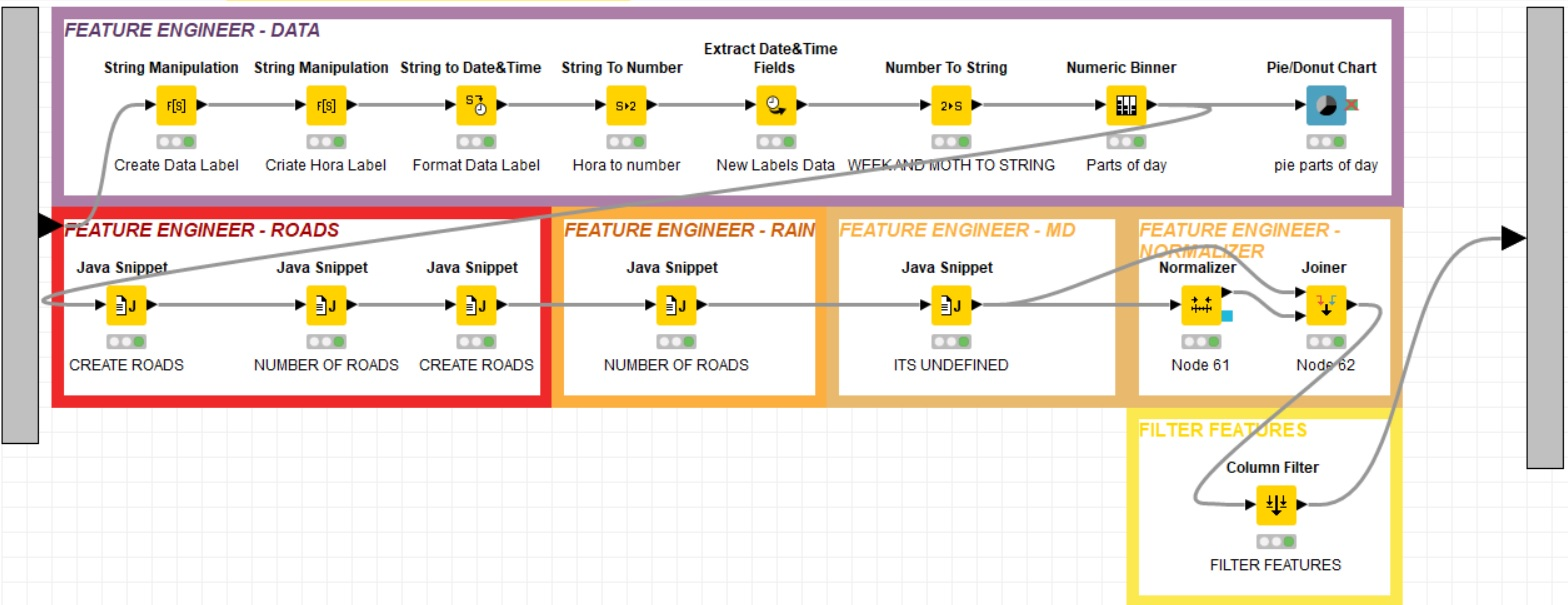
\includegraphics[width=\linewidth]{imagens/DATAPREPARATION.jpg}
  \caption{Workflow Data Preparation}
  \label{fig:DATAPREPARATION}
\end{figure}

As transformações de dados realizadas foram uteis para os resultados do modelo e foram suportadas pela analise de dados efetuada e explicada no capitulo anterior. 


Como se pode ver na figura em baixo, pode-se retirar várias informações de algumas features, como por exemplo da record\underline{ }date e da affected\underline{ }roads. Nesta forma inicial estas duas features não contém muita informação pertinente para o modelo. 

\begin{figure} [ h! ]
  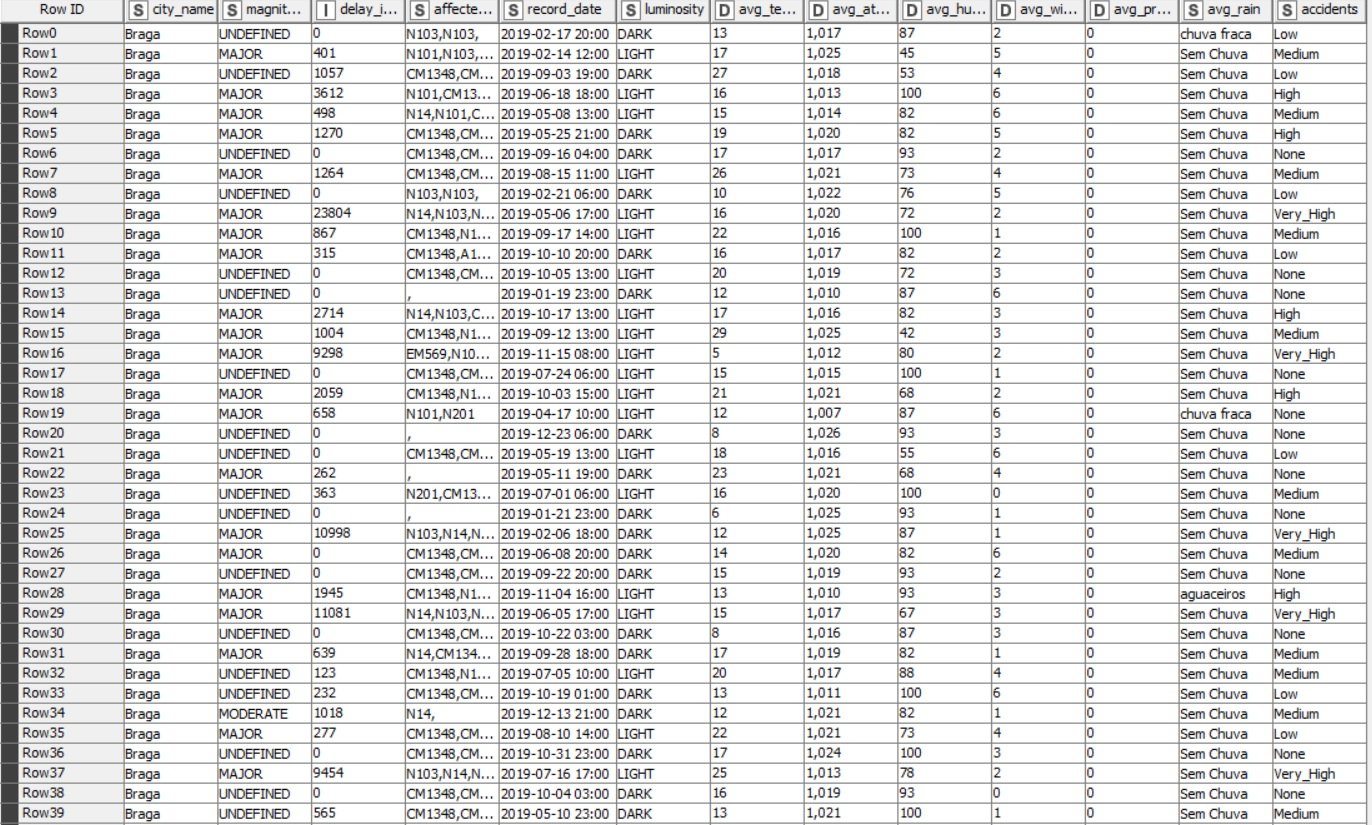
\includegraphics[width=\linewidth]{imagens/DATASET.jpg}
  \caption{Data Set}
  \label{fig:DATASET}
\end{figure}

A partir de técnicas de tratamento de dados foi possivel criar novas features geradas a partir de informação disponivel na feature record\underline{ }date, foi separada a data da hora em duas novas features, foi criada a nova coluna do trimestre e das semans, assim como o dia da semana e a parte do dia. 

\begin{figure} [ h! ]
  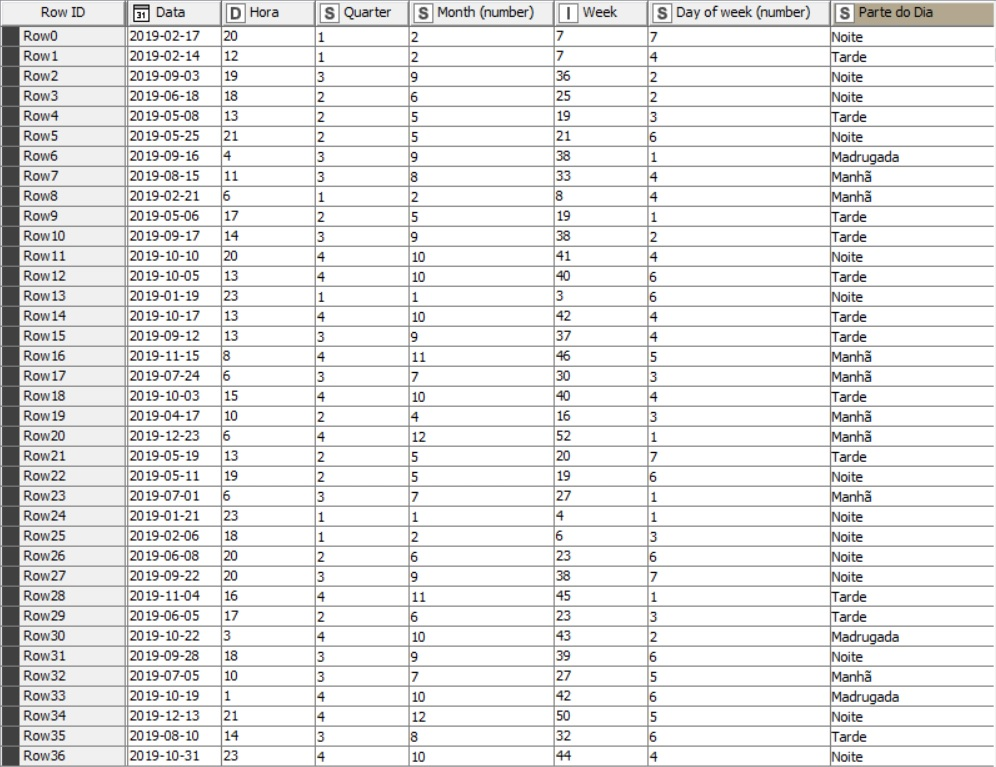
\includegraphics[width=\linewidth]{imagens/DATAFE.jpg}
  \caption{Novas Features geradas da \textbf{record\underline{ }date}}
  \label{fig:DATAFE}
\end{figure}
\newpage
A feature \textbf{Parte do Dia} foi concebida a partir da \textbf{Hora} e foram selecionados intervalos de forma a que cada parte do dia ficasse com frequencias identicas. 

\begin{figure} [ h! ]
  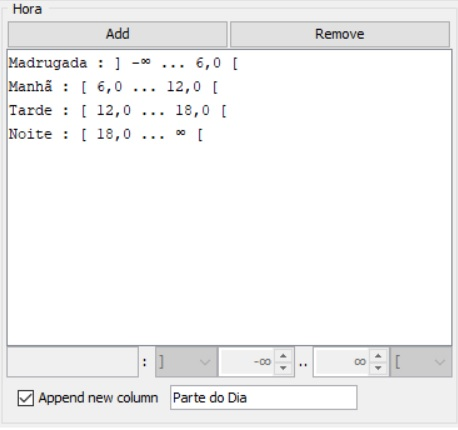
\includegraphics[width=\linewidth]{imagens/partedodiacode.jpg}
  \caption{Configuração da Feature \textbf{Parte do Dia}}
  \label{fig:partedodiacode}
\end{figure}

\begin{figure} [ h! ]
  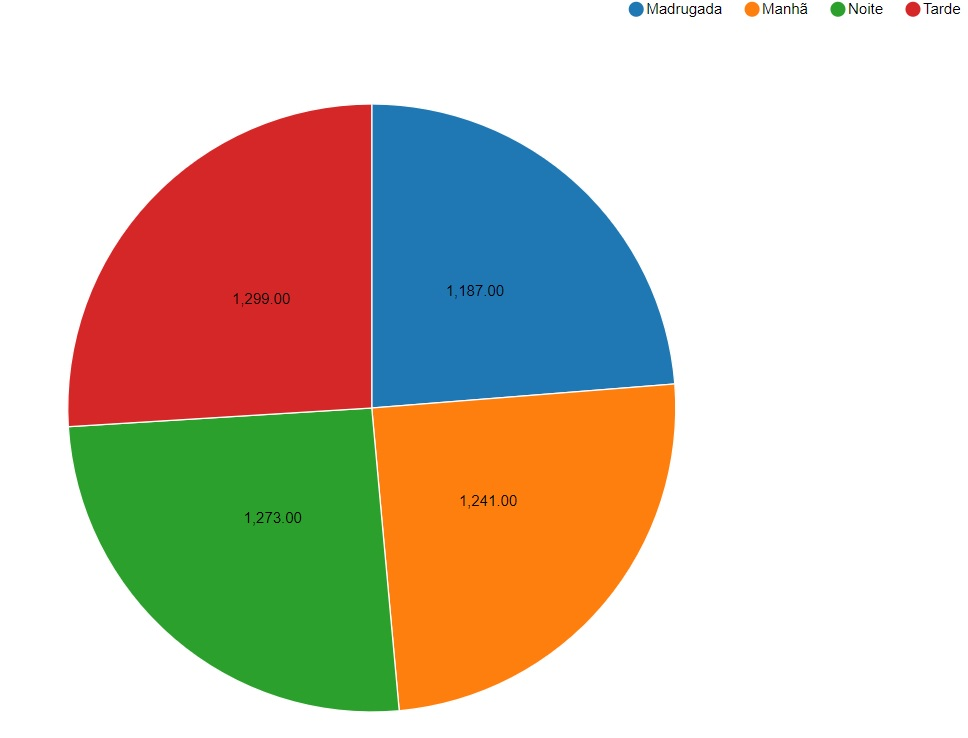
\includegraphics[width=\linewidth]{imagens/partedodiafreq.jpg}
  \caption{Distribuição da Feature \textbf{Parte do Dia}}
  \label{fig:partedodiafreq}
\end{figure}

Outra das transformações mais importantes foi sobre a feature {affected\underline{ }roads ...(CONTINUAR)




\newpage
\subsection{Modelação}
\subsection{Análise de Resultados}



\newpage
\section{DataSet 1}
\subsection{Contexto do Dataset}
\subsection{Análise e Compreensão dos Dados}
\subsection{Modelação}
\subsection{Análise de Resultados}
\section{Conclusão}

\end{document}
